% A skeleton file for producing Computer Engineering reports
% https://github.com/DeepHorizons/KGCOEReport_template

\documentclass[CMPE]{KGCOEReport}

% The following should be changed to represent your personal information
\newcommand{\classCode}{CMPE 460}  % 4 char code with number
\newcommand{\name}{Tevin Hendess and Adam Schultzer}
\newcommand{\LabSectionNum}{1}
\newcommand{\LabInstructor}{Stephanie Soldavini}
\newcommand{\TAs}{Caiden Merritt \\ Jack Milkovich \\ Oliver Vinneras}
\newcommand{\LectureSectionNum}{01}
\newcommand{\LectureInstructor}{Stephanie Soldavini}
\newcommand{\exerciseNumber}{6}
\newcommand{\exerciseDescription}{Motor Control}
\newcommand{\dateDone}{March 5th, 2025}
\newcommand{\dateSubmitted}{March 19th, 2025}

\begin{document}
\maketitle

\section*{Abstract}
The final autonomous car project will require a significant amount of fine
motor control to pilot the vehicle through the course. In order to prepare for
this challenge, the exercise involves programming and creating a hardware
environment for testing multiple motors and servos. Using a DC motor, stepper
motor, and a servo, the unique applications of each can be displayed while
also allowing for practice with PWM signals and the proper timing control of
the devices. Because all motors acted as expected, the exercise was a success. 

\section*{Circuit Schematics}
By using an H-bridge, a DC motor can be controlled by a microcontroller. A 
setup for this is demonstrated in Figure \ref{fig:hbridge}.
\begin{figure}[H]
    \centering
    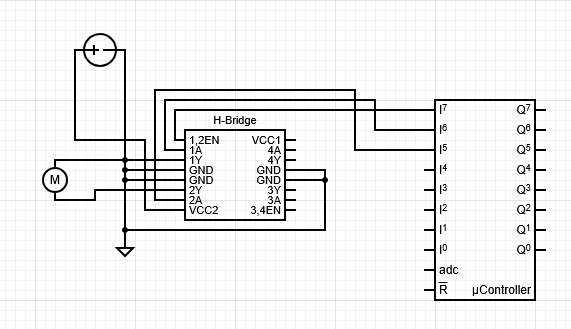
\includegraphics[width=1\textwidth]{Images/hbridge_diagram.png} % The width= allows you to change the image scaling
    \caption{\textit{Circuit Diagram of the H-Bridge Connections}}
    \label{fig:hbridge}
\end{figure}
In Figure \ref{fig:hbridge}, the microcontroller has three connections to the 
H-bridge. One is the 5V power from pin I7 which allows the IC to function. The
 other two, from pins I6 and I5, are the two PWM signals which actually 
 control the motor. However, because of the H-bridge, these signals do not 
 connect directly to the motor. Instead, they are interpreted and used to 
 control the supply of 10V power from the external power supply. In this way, 
 a microcontroller only capable of outputting 5V can run a much more powerful 
 motor. \\ \newpage

The servo connections are very straightforward and are shown in Figure 
\ref{fig:servo}.
\begin{figure}[H]
    \centering
    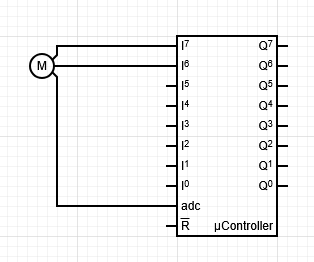
\includegraphics[width=1\textwidth]{Images/servo_diagram.png} % The width= allows you to change the image scaling
    \caption{\textit{Circuit Diagram of the Servo Connections}}
    \label{fig:servo}
\end{figure}
In Figure \ref{fig:servo} the microcontroller is the MSP432 with only one of 
its actual outputs being used (in this case I6 or what could be pin 5.6). The 
other two connections to the servo are simply the 5V power and GND which allow
 the device to function. Through this simple setup, the servo can be commanded
  to any position using the data connection.

\section*{Prelab Questions}
Part 1 \\
a) Maximum stall torque before reduction: 4.5kgcm/30 = 0.15kgcm = 2.083oz-in \\
b) max current draw = 1.4 A \\
c) max turn speed before reduction = 0.21 kRPM * 30 = 6.3 kRPM \\
d) maximum torque after reduction: 4.5kgcm = 62.49 oz-in \\
e) max turn speed after reduction = 0.21 kRPM \\

Part 2 \\
a) The diodes in this circuit provide a safe path for the current so that it 
doesn't go through the transistors and destroy them. 
This is particularly a problem when the power is removed from the motors and 
the voltage spikes. \\
b) The capacitor minimizes spikes both upwards and downwards. It can absorb 
voltage when it spikes and discharge 
energy when voltage dips. This can occur when there is a direct path from +V 
to ground. \\
c) By creating the H-bridge with two transistors, it is possible to control 
both the direction of the motor and supports separate 
driving and control voltages. This is very advantageous for many applications 
and helps make the circuit much more versatile. \\
d) Two different transistors are used because one is an NPN while the other is
a PNP. This means they are open or closed based 
on opposite voltages. It is this property and setup that allows for control of
the direction as a single voltage change can both 
open and close current paths. The different transistor models exist due to the
2N transistors having faster switching times
for lower power applications, and the TIP transistors can handle higher power 
applications. \\ \newpage


\section*{Oscilloscope Captures}
In order to drive the DC motor, PWM signals were generated on two different 
pins at a 20\% duty cycle. An oscilloscope capture of this input is shown in 
Figure \ref{fig:part1_1}. \\
\begin{figure}[H]
    \centering
    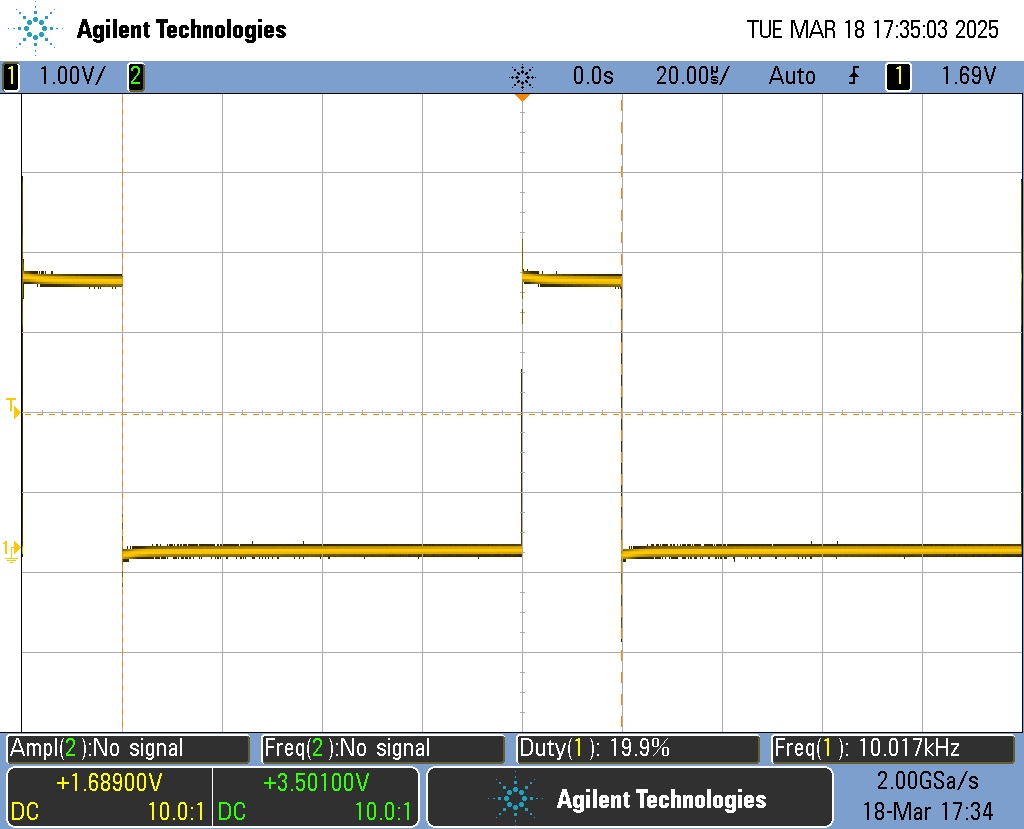
\includegraphics[width=1\textwidth]{Images/part1_1.png} % The width= allows you to change the image scaling
    \caption{\textit{The Oscilloscope Waveform of the 20\% Duty Cycle DC Motor}}
    \label{fig:part1_1}
\end{figure}
As shown in Figure \ref{fig:part1_1}, the input signal displayed on the 
waveform had a duty cycle of 20\%. This signal operated at a frequency of 10k 
Hz and would be high for 2000 Hz before dropping low for the remainder of the 
cycle. Figure \ref{fig:part1_1} displays two such cycles. At the end of each 
full cycle, the motor switches direction and spins the opposite way until it 
reverses again. This is a result of the PWM signals switching on and off with 
each one controlling a direction. \\ \newpage

When using the H-bridge, a smaller voltage signal is used to control the 
actual power signal. This relationship is shown in Figure \ref{fig:part1_2}.
\begin{figure}[H]
    \centering
    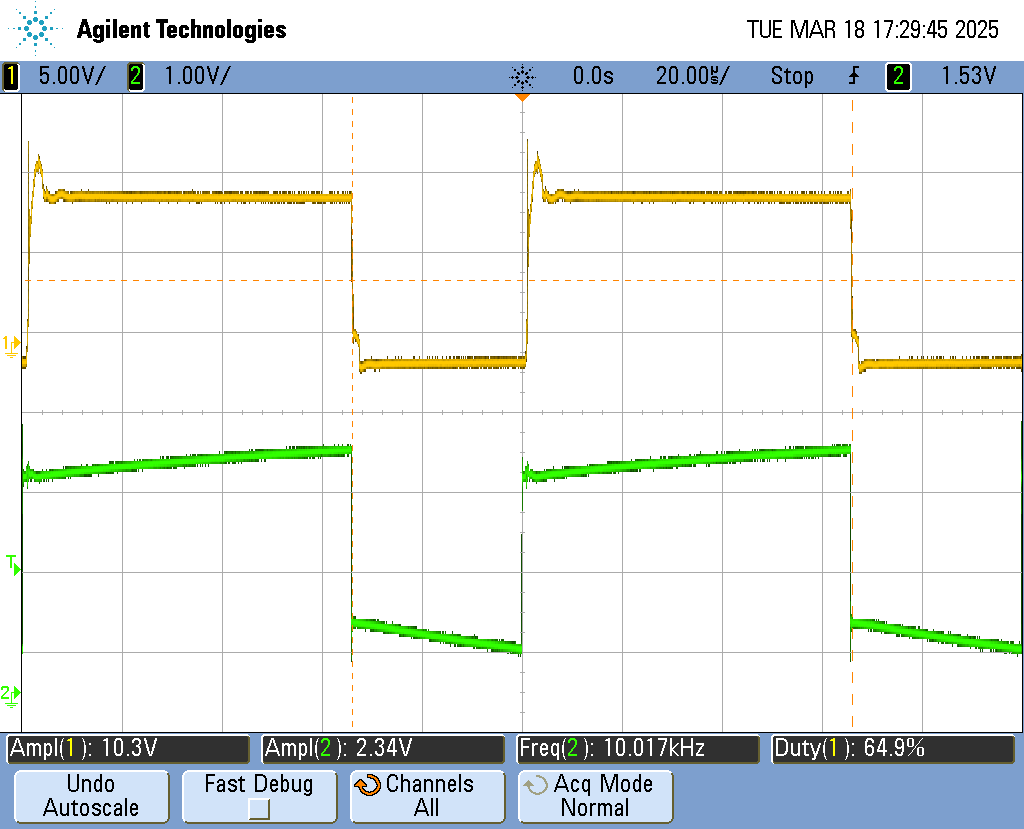
\includegraphics[width=1\textwidth]{Images/part1_2.png} % The width= allows you to change the image scaling
    \caption{\textit{The Oscilloscope Waveform of the H-Bridge Input and Output}}
    \label{fig:part1_2}
\end{figure}
There are two signals present in the oscilloscope capture displayed in Figure 
\ref{fig:part1_2}: the upper, yellow signal is the 10V output and the lower, 
green signal is the 3.3V input. Through the use of an H-bridge, the 3.3V 
output of the microcontroller is essentially mapped to the 10V source from the
 power supply which is actually driving the motor. In this way, the 
 microcontroller doesn't need to supply the high voltage required to achieve 
 higher torques on the motor. To change the speed of the motor, the voltage 
 output from the microcontroller can be adjusted which will in turn affect the
  voltage from the power supply to the motor. To change direction, the PWM 
  signals can be flipped and whichever was previously low goes high while that
   which was high goes low. Through this simple setup, a small microcontroller
    can completely control the DC motor.

\section*{Code Explanation}

\section*{Questions}
\setlength{\parindent}{20pt}
1. \underline{Explain how to change speed and direction of turn of the DC 
motor.} \\
\indent 
2. \underline{The above method requires two PWM lines, one for forward, and
one for reverse. Describe an alternate method that uses only one PWM line and
one GPIO line.} \\
\indent 
3. \underline{Which stepping mode does this code use?} \\
\indent 

\end{document}